\documentclass{standalone}
\usepackage{tikz}
\usetikzlibrary{shapes, arrows.meta}

\begin{document}

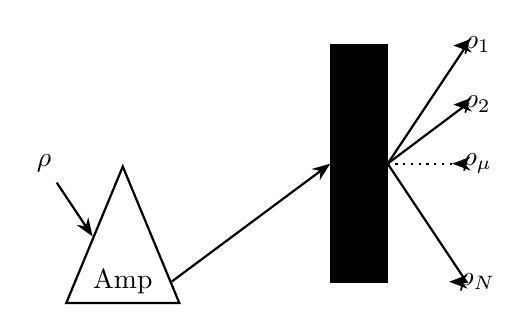
\begin{tikzpicture}[thick]

    % Amplifier
    \node[draw, isosceles triangle, shape border rotate=90, minimum width=1cm, minimum height=1cm, anchor=apex] (amp) at (0,0) {Amp};

    % Beam Splitter
    \node[draw, fill=black, minimum width=0.7cm, minimum height=3cm] (bs) at (3,0) {};

    % Initial state
    \node at (-1, 0) (rho) {$\rho$};
    \draw[-{Stealth}] (rho) -- (amp);

    % Output lines and labels
    \draw[-{Stealth}] (amp.east) -- (bs.west);

    \foreach \i/\y in {1/1.5, 2/0.75, N/-1.5} {
        \node at (4.5, \y) (rho\i) {$\rho_{\i}$};
        \draw[-{Stealth}] (bs.east) -- ++(1, \y) -- (rho\i);
    }

    % Dotted lines
    \node at (4.5, 0) (rhom) {$\rho_{\mu}$};
    \draw[dotted, -{Stealth}] (bs.east) -- ++(1, 0) -- (rhom);

\end{tikzpicture}

\end{document}